% AeroCast-AI -- Phase 2 report (IEEE conference format).
% Build: cd report && tectonic -X compile main.tex
% figures/ and tables/ are generated by scripts/export_report_assets.py from results/ (never edit by hand).
% The prose is hand-written; scripts/check_report_numbers.py asserts the quoted numbers against results/.
\documentclass[conference]{IEEEtran}
\usepackage[T1]{fontenc}
\usepackage{cite}
\usepackage{amsmath,amssymb}
\usepackage{graphicx}
\usepackage{booktabs}
\usepackage{array}
\usepackage[inline]{enumitem}
\usepackage{tikz}
\usetikzlibrary{positioning,arrows.meta,fit}
\usepackage[hidelinks]{hyperref}
\graphicspath{{figures/}}
\setlist[itemize]{leftmargin=1.1em,itemsep=1pt,topsep=2pt,parsep=0pt}
\newcommand{\tabsize}{\footnotesize}

\begin{document}

\title{Day-Ahead Flight Delay Risk, Phase 2:\\
Entity Embeddings, Causal History Sequences and a Wide \& Deep Hybrid}

\author{\IEEEauthorblockN{Nipun Patlori, Anushka Tyagi, Mohan Kumar C R, Omkar Hadole, Krish Dabas}
\IEEEauthorblockA{Team T49 --- Advanced Machine Learning, Semester 5 --- Project 21, Phase 2 (deep learning)}}

\maketitle

%%ABSTRACT%%

\begin{IEEEkeywords}
flight delay prediction, entity embeddings, recurrent neural networks, wide and deep learning, data leakage, calibration
\end{IEEEkeywords}

%====================================================================
\section{Introduction}\label{sec:intro}
Phase~1 built a leakage-tested day-ahead pipeline for flights leaving New York in 2013: at \textbf{20:00 on the evening before departure}, estimate the probability that a flight arrives at least 15 minutes late. A regularised logistic regression (LogReg) on 43 hand-built schedule, congestion, calendar and past-delay features was selected by rolling-origin cross-validation (CV), ahead of XGBoost. The brief for Phase~2 names the gap this leaves: \emph{manual route and congestion summaries may miss complex interactions between time, airport, carrier and recent delay dynamics}.
\begin{itemize}
\item \textbf{Question.} Can networks that \emph{learn} representations---embeddings for airlines and airports, a recurrent encoder over recent delay history---recover signal the hand-built features miss, under exactly the same decision clock, data, splits and folds?
\item \textbf{Fair comparison.} Every Phase~2 input is built from information known at 20:00 on $D-1$, every model is selected on the Phase~1 folds, and the selection, calibration and rescheduling rules were committed before any Phase~2 model was trained (Sec.~\ref{sec:protocol}).
\end{itemize}

\textbf{Contributions.}
\begin{itemize}
\item An \textbf{embedding MLP} (the brief's required model) and a \textbf{GRU over causal daily history windows}, whose inputs reproduce the Phase~1 history features exactly and pass the Phase~1 leakage tests.
\item A \textbf{Wide \& Deep hybrid} whose wide part \emph{is} the Phase~1 LogReg at initialisation, so the network can only add to the ML model; and a secondary hybrid that feeds learned embeddings to XGBoost.
\item \textbf{Ablations and diagnostics} on CV that explain where the networks gain and lose, including a procedural error found and corrected before any test evaluation.
\item \textbf{Calibrated} probabilities under seasonal shift and an \textbf{offline what-if rescheduling} analysis under explicit assumptions.
\end{itemize}

%====================================================================
\section{Deep-Learning Literature Review}\label{sec:related}
\begin{itemize}
\item \textbf{Entity embeddings.} Guo and Berkhahn~\cite{guo2016entity} map each categorical value to a learned dense vector trained with the supervised loss; compared with one-hot inputs this reduces parameters and helps most for high-cardinality variables, and the learned distances can be visualised. We use them for carrier, origin and destination, and test tail and flight identifiers as an ablation.
\item \textbf{Deep learning on tabular data.} Gorishniy et al.~\cite{gorishniy2021revisiting} find that a well-tuned MLP or ResNet is a strong baseline but no architecture dominates gradient-boosted trees. Grinsztajn et al.~\cite{grinsztajn2022tree} explain why trees still win on typical medium-sized tabular data: networks are biased towards smooth functions, are hurt by uninformative features and are not rotation-invariant in the right way. Both predict that our networks will struggle to beat a strong tabular model; we test this directly.
\item \textbf{Flight delays with deep learning.} Kim et al.~\cite{kim2016deep} combine recurrent networks (LSTM, deep RNN) over sequences of airport delay states to predict flight delays. Their sequences are built from observed delay states; our GRU instead reads windows that end at the decision clock, so that a day-ahead prediction never sees the day it predicts.
\item \textbf{Recurrent encoders.} The gated recurrent unit (GRU) of Cho et al.~\cite{cho2014gru} keeps a hidden state updated through reset and update gates, which lets a small model weight recent days more than old ones without fixing the weights by hand.
\item \textbf{Wide \& Deep.} Cheng et al.~\cite{cheng2016wide} jointly train a linear model on (cross-)features (memorisation) and a deep network on embeddings (generalisation), summing their logits. Our wide part is the Phase~1 LogReg itself.
\item \textbf{Regularisation and training.} Dropout~\cite{srivastava2014dropout}, decoupled weight decay (AdamW)~\cite{loshchilov2019adamw} and layer normalisation~\cite{ba2016layernorm}, which normalises within a row and so never couples rows of a batch. Seed ensembles~\cite{lakshminarayanan2017ensembles} average independently trained networks.
\item \textbf{Calibration and leakage.} Guo et al.~\cite{guo2017calibration} show that modern networks are often over-confident and introduce \emph{temperature scaling}; Kaufman et al.~\cite{kaufman2012leakage} define leakage as using information unavailable at prediction time, which our decision clock rules out.
\end{itemize}

%====================================================================
\section{Data, Decision Clock and Network Inputs}\label{sec:data}
\begin{itemize}
\item \textbf{Same data and split as Phase~1.} \texttt{nycflights13}: departures from EWR, JFK and LGA in 2013. Target $y=\mathbb{1}[\text{arrival delay}\ge 15]$; cancelled and diverted flights excluded. Train 8~Jan--31~Aug, calibration Sep--Oct, test Nov--Dec; rolling-origin CV inside train with validation months May, June, July and August.
\item \textbf{Decision clock.} An outcome may feed an input for day $D$ only once it is known by 20:00 on $D-1$: a delay at gate arrival, a cancellation at departure. Phase~2 imports this code from Phase~1 rather than re-implementing it.
\item \textbf{Tabular inputs.} The 3 categorical and 40 numeric Phase~1 features. Category vocabularies (a shared index for values with fewer than 50 fitting rows, as Phase~1's one-hot encoder), imputation medians and the scaler are fitted on each model's own fitting rows only.
\item \textbf{Fitting clock.} The final networks are fitted for 1~September on the %%FITROWS%% training rows whose labels were known by then (%%EXCLUDED%% late-August rows are excluded, as in Phase~1).
\end{itemize}

%====================================================================
\section{Architecture}\label{sec:arch}
\begin{figure}[t]
\centering
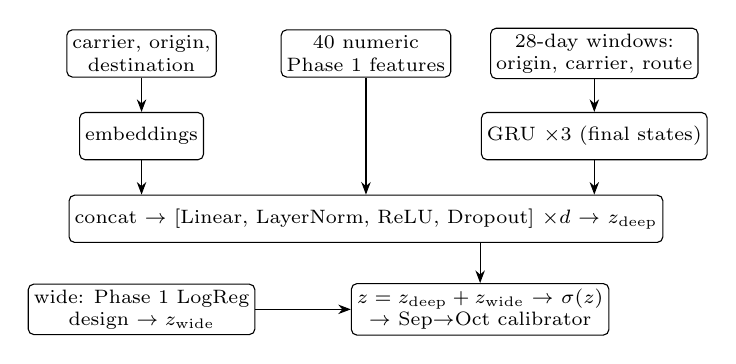
\begin{tikzpicture}[font=\scriptsize,
  box/.style={draw, rounded corners=2pt, align=center, minimum height=6mm, inner sep=2pt},
  arr/.style={-{Stealth[length=1.6mm]}}]
\node[box] (cat) at (0,0) {carrier, origin,\\destination};
\node[box] (num) at (2.85,0) {40 numeric\\Phase 1 features};
\node[box] (seq) at (5.75,0) {28-day windows:\\origin, carrier, route};
\node[box] (emb) at (0,-1.05) {embeddings};
\node[box] (gru) at (5.75,-1.05) {GRU $\times 3$ (final states)};
\node[box, minimum width=52mm] (mlp) at (2.85,-2.1) {concat $\rightarrow$ [Linear, LayerNorm, ReLU, Dropout] $\times d$ $\rightarrow$ $z_{\text{deep}}$};
\node[box] (wide) at (0,-3.25) {wide: Phase 1 LogReg\\design $\rightarrow z_{\text{wide}}$};
\node[box] (sum) at (4.3,-3.25) {$z=z_{\text{deep}}+z_{\text{wide}}$ $\rightarrow$ $\sigma(z)$\\$\rightarrow$ Sep$\rightarrow$Oct calibrator};
\draw[arr] (cat) -- (emb); \draw[arr] (seq) -- (gru);
\draw[arr] (emb) -- (emb |- mlp.north); \draw[arr] (num) -- (mlp); \draw[arr] (gru) -- (gru |- mlp.north);
\draw[arr] (mlp.south -| sum) -- (sum); \draw[arr] (wide) -- (sum);
\end{tikzpicture}
\caption{Phase~2 networks. The MLP uses the embedding and numeric branches; the GRU model adds the history branch; Wide \& Deep adds the wide branch, initialised to the Phase~1 LogReg with the deep head at zero.}
\label{fig:arch}
\end{figure}
\begin{itemize}
\item \textbf{Embedding MLP.} Each categorical value gets a vector of width $\min(16, \lceil 1.6\,n^{0.56}\rceil)$ for a vocabulary of size $n$; vectors and the 40 standardised numerics are concatenated and passed through $d$ blocks of Linear, LayerNorm, ReLU and Dropout to a scalar logit (Fig.~\ref{fig:arch}).
\item \textbf{GRU history model.} For each entity type (origin, carrier, route) and target date $D$, a window of the last 28 \emph{availability days} holds, per day, the known arrivals, late arrivals, total delay minutes, known departures and cancellations, transformed to log counts and rates. One GRU per entity type reads its window oldest day first; the final hidden states join the MLP input.
\item \textbf{Wide \& Deep.} The wide part is a linear layer on the Phase~1 LogReg design matrix (one-hot categoricals and standardised numerics), initialised from the LogReg fitted on the same rows; the deep part is the better of the MLP and the GRU model, with its output layer initialised to zero. Both parts are trained jointly.
\item \textbf{Embeddings $\rightarrow$ XGBoost.} The MLP's carrier, origin and destination vectors are appended to the Phase~1 XGBoost features (same configuration and tree count).
\end{itemize}

%====================================================================
\section{Theory}\label{sec:theory}
\begin{itemize}
\item \textbf{Embeddings are a factorised one-hot layer.} For a one-hot vector $e_c$ and first-layer weights $W\in\mathbb{R}^{h\times n}$, $We_c$ is column $c$ of $W$. An embedding writes $W=UE$ with $E\in\mathbb{R}^{k\times n}$, $k\ll n$: categories share the $k$ directions, so a rare value borrows strength from similar ones, and parameters fall from $hn$ to $kn+hk$.
\item \textbf{GRU.} With input $x_t$ and state $h_{t-1}$:
$z_t=\sigma(W_zx_t+U_zh_{t-1})$, $r_t=\sigma(W_rx_t+U_rh_{t-1})$, $\tilde h_t=\tanh(Wx_t+U(r_t\odot h_{t-1}))$, $h_t=(1-z_t)\odot h_{t-1}+z_t\odot\tilde h_t$.
A Phase~1 $w$-day history feature is a fixed sum over the last $w$ slots of the same window; the GRU can represent such sums and also learn recency weights and non-linear trends.
\item \textbf{Wide \& Deep starts at LogReg.} With the deep head at zero, $z(x)=w^\top\phi(x)+b$, the fitted LogReg. Joint training minimises
$\mathcal{L}=\frac1N\sum_i \ell\bigl(y_i,\,w^\top\phi(x_i)+b+f_\theta(x_i)\bigr)+\lambda\|\theta\|^2$,
so $f_\theta$ learns a residual correction in the logit, as one step of functional gradient boosting with a network as the base learner.
\item \textbf{Loss without class weights.} Binary cross-entropy is a proper scoring rule: its minimiser is the true probability. Weighting positives by $\omega$ shifts the optimal logit by $\log\omega$, so it would mis-calibrate every prediction; imbalance is handled by the operating policy instead.
\item \textbf{Temperature vs Platt.} Temperature scaling $q=\sigma(z/T)$ keeps the ranking and fixes over- or under-confidence, but has no intercept: it cannot move the mean prediction to a new base rate. Platt scaling $q=\sigma(az+b)$ can. Our seasons shift the base rate (calibration months 15.7\% late, test 25.8\%), so Platt-type calibrators are expected to win; we test both.
\item \textbf{Seed ensembles.} Averaging the logits of $M$ networks trained from different seeds reduces the variance term of the error by up to a factor $M$ when their errors are weakly correlated~\cite{lakshminarayanan2017ensembles}.
\end{itemize}

%====================================================================
\section{Training, Validation and Leakage Protocol}\label{sec:protocol}
\begin{itemize}
\item \textbf{Pre-registration.} The protocol (selection rules, search budgets, calibrator rule, test lock) was committed to the repository before any model was trained; every later amendment is in a dated change log with its reason.
\item \textbf{Optimisation.} AdamW, batch 1024, binary cross-entropy, at most 40 epochs.
\item \textbf{Early stopping as deployed.} In each fold, the last 14 days of the training window form an inner holdout that only chooses the number of epochs (patience 4, log loss); the network is then \textbf{refitted on all of the fold's rows} for that many epochs and scored once on the validation month. The final model repeats this with the mean CV epoch count. The validation month never chooses anything.
\item \textbf{Search and seeds.} 20 random MLP configurations, 12 GRU and 12 Wide \& Deep configurations, each scored on CV with one seed; the best of each family is re-scored as a 5-seed ensemble (mean logit), which is the number used for selection.
\item \textbf{Final-model rule.} Highest mean CV AP as deployed among the Phase~1 and Phase~2 models; within 0.005 of the best, the one with fewer parameters.
\item \textbf{Leakage tests.} %%NTESTS%% automated tests. The GRU windows reproduce the Phase~1 history counts exactly for every flight and window length; randomising future outcomes, late-evening $D-1$ arrivals or same-day cancellations leaves day-$D$ inputs unchanged, each with a positive control; encoders ignore every calibration and test row; test labels load only in the final stage and only with the protocol committed. Deliberately bucketing outcomes by flight date instead of availability date fails 13 of these checks.
\end{itemize}

%%RESULTS%%

\bibliographystyle{IEEEtran}
\bibliography{references}

\end{document}
